% Created by tikzDevice version 0.10.1.2 on 2018-02-15 11:51:08
% !TEX encoding = UTF-8 Unicode
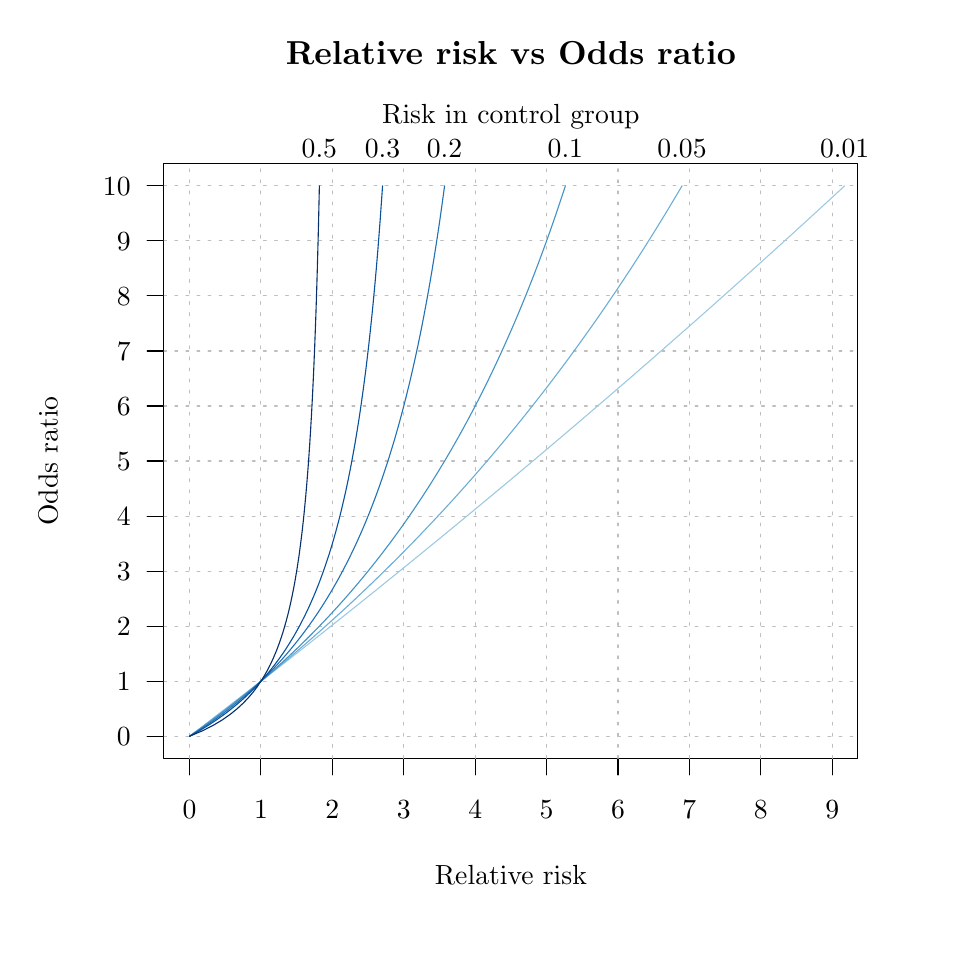
\begin{tikzpicture}[x=1pt,y=1pt]
\definecolor{fillColor}{RGB}{255,255,255}
\path[use as bounding box,fill=fillColor,fill opacity=0.00] (0,0) rectangle (325.21,325.21);
\begin{scope}
\path[clip] (  0.00,  0.00) rectangle (325.21,325.21);
\definecolor{drawColor}{RGB}{0,0,0}

\path[draw=drawColor,line width= 0.4pt,line join=round,line cap=round] ( 49.20, 61.20) --
	(300.01, 61.20) --
	(300.01,276.01) --
	( 49.20,276.01) --
	( 49.20, 61.20);
\end{scope}
\begin{scope}
\path[clip] (  0.00,  0.00) rectangle (325.21,325.21);
\definecolor{drawColor}{RGB}{0,0,0}

\node[text=drawColor,anchor=base,inner sep=0pt, outer sep=0pt, scale=  1.00] at (174.61, 15.60) {Relative risk};

\node[text=drawColor,rotate= 90.00,anchor=base,inner sep=0pt, outer sep=0pt, scale=  1.00] at ( 10.80,168.61) {Odds ratio};
\end{scope}
\begin{scope}
\path[clip] (  0.00,  0.00) rectangle (325.21,325.21);
\definecolor{drawColor}{RGB}{0,0,0}

\path[draw=drawColor,line width= 0.4pt,line join=round,line cap=round] ( 49.20, 69.16) -- ( 49.20,268.06);

\path[draw=drawColor,line width= 0.4pt,line join=round,line cap=round] ( 49.20, 69.16) -- ( 43.20, 69.16);

\path[draw=drawColor,line width= 0.4pt,line join=round,line cap=round] ( 49.20, 89.05) -- ( 43.20, 89.05);

\path[draw=drawColor,line width= 0.4pt,line join=round,line cap=round] ( 49.20,108.94) -- ( 43.20,108.94);

\path[draw=drawColor,line width= 0.4pt,line join=round,line cap=round] ( 49.20,128.83) -- ( 43.20,128.83);

\path[draw=drawColor,line width= 0.4pt,line join=round,line cap=round] ( 49.20,148.72) -- ( 43.20,148.72);

\path[draw=drawColor,line width= 0.4pt,line join=round,line cap=round] ( 49.20,168.61) -- ( 43.20,168.61);

\path[draw=drawColor,line width= 0.4pt,line join=round,line cap=round] ( 49.20,188.50) -- ( 43.20,188.50);

\path[draw=drawColor,line width= 0.4pt,line join=round,line cap=round] ( 49.20,208.39) -- ( 43.20,208.39);

\path[draw=drawColor,line width= 0.4pt,line join=round,line cap=round] ( 49.20,228.28) -- ( 43.20,228.28);

\path[draw=drawColor,line width= 0.4pt,line join=round,line cap=round] ( 49.20,248.17) -- ( 43.20,248.17);

\path[draw=drawColor,line width= 0.4pt,line join=round,line cap=round] ( 49.20,268.06) -- ( 43.20,268.06);

\node[text=drawColor,anchor=base east,inner sep=0pt, outer sep=0pt, scale=  1.00] at ( 37.20, 65.71) {0};

\node[text=drawColor,anchor=base east,inner sep=0pt, outer sep=0pt, scale=  1.00] at ( 37.20, 85.60) {1};

\node[text=drawColor,anchor=base east,inner sep=0pt, outer sep=0pt, scale=  1.00] at ( 37.20,105.49) {2};

\node[text=drawColor,anchor=base east,inner sep=0pt, outer sep=0pt, scale=  1.00] at ( 37.20,125.38) {3};

\node[text=drawColor,anchor=base east,inner sep=0pt, outer sep=0pt, scale=  1.00] at ( 37.20,145.27) {4};

\node[text=drawColor,anchor=base east,inner sep=0pt, outer sep=0pt, scale=  1.00] at ( 37.20,165.16) {5};

\node[text=drawColor,anchor=base east,inner sep=0pt, outer sep=0pt, scale=  1.00] at ( 37.20,185.05) {6};

\node[text=drawColor,anchor=base east,inner sep=0pt, outer sep=0pt, scale=  1.00] at ( 37.20,204.94) {7};

\node[text=drawColor,anchor=base east,inner sep=0pt, outer sep=0pt, scale=  1.00] at ( 37.20,224.83) {8};

\node[text=drawColor,anchor=base east,inner sep=0pt, outer sep=0pt, scale=  1.00] at ( 37.20,244.73) {9};

\node[text=drawColor,anchor=base east,inner sep=0pt, outer sep=0pt, scale=  1.00] at ( 37.20,264.62) {10};

\path[draw=drawColor,line width= 0.4pt,line join=round,line cap=round] ( 58.49, 61.20) -- (290.73, 61.20);

\path[draw=drawColor,line width= 0.4pt,line join=round,line cap=round] ( 58.49, 61.20) -- ( 58.49, 55.20);

\path[draw=drawColor,line width= 0.4pt,line join=round,line cap=round] ( 84.29, 61.20) -- ( 84.29, 55.20);

\path[draw=drawColor,line width= 0.4pt,line join=round,line cap=round] (110.10, 61.20) -- (110.10, 55.20);

\path[draw=drawColor,line width= 0.4pt,line join=round,line cap=round] (135.90, 61.20) -- (135.90, 55.20);

\path[draw=drawColor,line width= 0.4pt,line join=round,line cap=round] (161.71, 61.20) -- (161.71, 55.20);

\path[draw=drawColor,line width= 0.4pt,line join=round,line cap=round] (187.51, 61.20) -- (187.51, 55.20);

\path[draw=drawColor,line width= 0.4pt,line join=round,line cap=round] (213.31, 61.20) -- (213.31, 55.20);

\path[draw=drawColor,line width= 0.4pt,line join=round,line cap=round] (239.12, 61.20) -- (239.12, 55.20);

\path[draw=drawColor,line width= 0.4pt,line join=round,line cap=round] (264.92, 61.20) -- (264.92, 55.20);

\path[draw=drawColor,line width= 0.4pt,line join=round,line cap=round] (290.73, 61.20) -- (290.73, 55.20);

\node[text=drawColor,anchor=base,inner sep=0pt, outer sep=0pt, scale=  1.00] at ( 58.49, 39.60) {0};

\node[text=drawColor,anchor=base,inner sep=0pt, outer sep=0pt, scale=  1.00] at ( 84.29, 39.60) {1};

\node[text=drawColor,anchor=base,inner sep=0pt, outer sep=0pt, scale=  1.00] at (110.10, 39.60) {2};

\node[text=drawColor,anchor=base,inner sep=0pt, outer sep=0pt, scale=  1.00] at (135.90, 39.60) {3};

\node[text=drawColor,anchor=base,inner sep=0pt, outer sep=0pt, scale=  1.00] at (161.71, 39.60) {4};

\node[text=drawColor,anchor=base,inner sep=0pt, outer sep=0pt, scale=  1.00] at (187.51, 39.60) {5};

\node[text=drawColor,anchor=base,inner sep=0pt, outer sep=0pt, scale=  1.00] at (213.31, 39.60) {6};

\node[text=drawColor,anchor=base,inner sep=0pt, outer sep=0pt, scale=  1.00] at (239.12, 39.60) {7};

\node[text=drawColor,anchor=base,inner sep=0pt, outer sep=0pt, scale=  1.00] at (264.92, 39.60) {8};

\node[text=drawColor,anchor=base,inner sep=0pt, outer sep=0pt, scale=  1.00] at (290.73, 39.60) {9};
\end{scope}
\begin{scope}
\path[clip] ( 49.20, 61.20) rectangle (300.01,276.01);
\definecolor{drawColor}{RGB}{190,190,190}

\path[draw=drawColor,line width= 0.4pt,dash pattern=on 1pt off 3pt ,line join=round,line cap=round] ( 49.20, 69.16) -- (300.01, 69.16);

\path[draw=drawColor,line width= 0.4pt,dash pattern=on 1pt off 3pt ,line join=round,line cap=round] ( 49.20, 89.05) -- (300.01, 89.05);

\path[draw=drawColor,line width= 0.4pt,dash pattern=on 1pt off 3pt ,line join=round,line cap=round] ( 49.20,108.94) -- (300.01,108.94);

\path[draw=drawColor,line width= 0.4pt,dash pattern=on 1pt off 3pt ,line join=round,line cap=round] ( 49.20,128.83) -- (300.01,128.83);

\path[draw=drawColor,line width= 0.4pt,dash pattern=on 1pt off 3pt ,line join=round,line cap=round] ( 49.20,148.72) -- (300.01,148.72);

\path[draw=drawColor,line width= 0.4pt,dash pattern=on 1pt off 3pt ,line join=round,line cap=round] ( 49.20,168.61) -- (300.01,168.61);

\path[draw=drawColor,line width= 0.4pt,dash pattern=on 1pt off 3pt ,line join=round,line cap=round] ( 49.20,188.50) -- (300.01,188.50);

\path[draw=drawColor,line width= 0.4pt,dash pattern=on 1pt off 3pt ,line join=round,line cap=round] ( 49.20,208.39) -- (300.01,208.39);

\path[draw=drawColor,line width= 0.4pt,dash pattern=on 1pt off 3pt ,line join=round,line cap=round] ( 49.20,228.28) -- (300.01,228.28);

\path[draw=drawColor,line width= 0.4pt,dash pattern=on 1pt off 3pt ,line join=round,line cap=round] ( 49.20,248.17) -- (300.01,248.17);

\path[draw=drawColor,line width= 0.4pt,dash pattern=on 1pt off 3pt ,line join=round,line cap=round] ( 49.20,268.06) -- (300.01,268.06);

\path[draw=drawColor,line width= 0.4pt,dash pattern=on 1pt off 3pt ,line join=round,line cap=round] ( 58.49, 61.20) -- ( 58.49,276.01);

\path[draw=drawColor,line width= 0.4pt,dash pattern=on 1pt off 3pt ,line join=round,line cap=round] ( 84.29, 61.20) -- ( 84.29,276.01);

\path[draw=drawColor,line width= 0.4pt,dash pattern=on 1pt off 3pt ,line join=round,line cap=round] (110.10, 61.20) -- (110.10,276.01);

\path[draw=drawColor,line width= 0.4pt,dash pattern=on 1pt off 3pt ,line join=round,line cap=round] (135.90, 61.20) -- (135.90,276.01);

\path[draw=drawColor,line width= 0.4pt,dash pattern=on 1pt off 3pt ,line join=round,line cap=round] (161.71, 61.20) -- (161.71,276.01);

\path[draw=drawColor,line width= 0.4pt,dash pattern=on 1pt off 3pt ,line join=round,line cap=round] (187.51, 61.20) -- (187.51,276.01);

\path[draw=drawColor,line width= 0.4pt,dash pattern=on 1pt off 3pt ,line join=round,line cap=round] (213.31, 61.20) -- (213.31,276.01);

\path[draw=drawColor,line width= 0.4pt,dash pattern=on 1pt off 3pt ,line join=round,line cap=round] (239.12, 61.20) -- (239.12,276.01);

\path[draw=drawColor,line width= 0.4pt,dash pattern=on 1pt off 3pt ,line join=round,line cap=round] (264.92, 61.20) -- (264.92,276.01);

\path[draw=drawColor,line width= 0.4pt,dash pattern=on 1pt off 3pt ,line join=round,line cap=round] (290.73, 61.20) -- (290.73,276.01);
\end{scope}
\begin{scope}
\path[clip] (  0.00,  0.00) rectangle (325.21,325.21);
\definecolor{drawColor}{RGB}{0,0,0}

\node[text=drawColor,anchor=base,inner sep=0pt, outer sep=0pt, scale=  1.20] at (174.61,312.01) {\bfseries Relative risk vs Odds ratio};
\end{scope}
\begin{scope}
\path[clip] ( 49.20, 61.20) rectangle (300.01,276.01);
\definecolor{drawColor}{RGB}{158,202,225}

\path[draw=drawColor,line width= 0.4pt,line join=round,line cap=round] ( 58.49, 69.16) --
	( 61.09, 71.15) --
	( 63.69, 73.13) --
	( 66.29, 75.12) --
	( 68.87, 77.11) --
	( 71.46, 79.10) --
	( 74.03, 81.09) --
	( 76.61, 83.08) --
	( 79.17, 85.07) --
	( 81.74, 87.06) --
	( 84.29, 89.05) --
	( 86.85, 91.04) --
	( 89.39, 93.02) --
	( 91.93, 95.01) --
	( 94.47, 97.00) --
	( 97.00, 98.99) --
	( 99.53,100.98) --
	(102.05,102.97) --
	(104.57,104.96) --
	(107.08,106.95) --
	(109.59,108.94) --
	(112.09,110.93) --
	(114.59,112.91) --
	(117.08,114.90) --
	(119.56,116.89) --
	(122.05,118.88) --
	(124.52,120.87) --
	(127.00,122.86) --
	(129.46,124.85) --
	(131.93,126.84) --
	(134.38,128.83) --
	(136.84,130.82) --
	(139.28,132.80) --
	(141.73,134.79) --
	(144.17,136.78) --
	(146.60,138.77) --
	(149.03,140.76) --
	(151.45,142.75) --
	(153.87,144.74) --
	(156.29,146.73) --
	(158.70,148.72) --
	(161.10,150.71) --
	(163.51,152.70) --
	(165.90,154.68) --
	(168.29,156.67) --
	(170.68,158.66) --
	(173.06,160.65) --
	(175.44,162.64) --
	(177.81,164.63) --
	(180.18,166.62) --
	(182.55,168.61) --
	(184.91,170.60) --
	(187.26,172.59) --
	(189.61,174.57) --
	(191.96,176.56) --
	(194.30,178.55) --
	(196.64,180.54) --
	(198.97,182.53) --
	(201.30,184.52) --
	(203.62,186.51) --
	(205.94,188.50) --
	(208.26,190.49) --
	(210.57,192.48) --
	(212.87,194.46) --
	(215.17,196.45) --
	(217.47,198.44) --
	(219.76,200.43) --
	(222.05,202.42) --
	(224.34,204.41) --
	(226.62,206.40) --
	(228.89,208.39) --
	(231.16,210.38) --
	(233.43,212.37) --
	(235.69,214.36) --
	(237.95,216.34) --
	(240.21,218.33) --
	(242.46,220.32) --
	(244.70,222.31) --
	(246.95,224.30) --
	(249.18,226.29) --
	(251.42,228.28) --
	(253.65,230.27) --
	(255.87,232.26) --
	(258.09,234.25) --
	(260.31,236.23) --
	(262.52,238.22) --
	(264.73,240.21) --
	(266.93,242.20) --
	(269.13,244.19) --
	(271.33,246.18) --
	(273.52,248.17) --
	(275.71,250.16) --
	(277.90,252.15) --
	(280.08,254.14) --
	(282.25,256.12) --
	(284.42,258.11) --
	(286.59,260.10) --
	(288.76,262.09) --
	(290.92,264.08) --
	(293.07,266.07) --
	(295.22,268.06);
\end{scope}
\begin{scope}
\path[clip] (  0.00,  0.00) rectangle (325.21,325.21);
\definecolor{drawColor}{RGB}{0,0,0}

\node[text=drawColor,anchor=base,inner sep=0pt, outer sep=0pt, scale=  1.00] at (295.22,278.42) {0.01};
\end{scope}
\begin{scope}
\path[clip] ( 49.20, 61.20) rectangle (300.01,276.01);
\definecolor{drawColor}{RGB}{107,174,214}

\path[draw=drawColor,line width= 0.4pt,line join=round,line cap=round] ( 58.49, 69.16) --
	( 61.19, 71.15) --
	( 63.87, 73.13) --
	( 66.51, 75.12) --
	( 69.13, 77.11) --
	( 71.72, 79.10) --
	( 74.29, 81.09) --
	( 76.83, 83.08) --
	( 79.34, 85.07) --
	( 81.83, 87.06) --
	( 84.29, 89.05) --
	( 86.73, 91.04) --
	( 89.15, 93.02) --
	( 91.54, 95.01) --
	( 93.91, 97.00) --
	( 96.25, 98.99) --
	( 98.57,100.98) --
	(100.87,102.97) --
	(103.15,104.96) --
	(105.41,106.95) --
	(107.64,108.94) --
	(109.85,110.93) --
	(112.04,112.91) --
	(114.22,114.90) --
	(116.37,116.89) --
	(118.50,118.88) --
	(120.61,120.87) --
	(122.70,122.86) --
	(124.77,124.85) --
	(126.83,126.84) --
	(128.86,128.83) --
	(130.88,130.82) --
	(132.88,132.80) --
	(134.86,134.79) --
	(136.82,136.78) --
	(138.77,138.77) --
	(140.70,140.76) --
	(142.61,142.75) --
	(144.50,144.74) --
	(146.38,146.73) --
	(148.24,148.72) --
	(150.09,150.71) --
	(151.92,152.70) --
	(153.73,154.68) --
	(155.53,156.67) --
	(157.31,158.66) --
	(159.08,160.65) --
	(160.83,162.64) --
	(162.57,164.63) --
	(164.30,166.62) --
	(166.01,168.61) --
	(167.70,170.60) --
	(169.38,172.59) --
	(171.05,174.57) --
	(172.70,176.56) --
	(174.34,178.55) --
	(175.97,180.54) --
	(177.58,182.53) --
	(179.19,184.52) --
	(180.77,186.51) --
	(182.35,188.50) --
	(183.91,190.49) --
	(185.46,192.48) --
	(187.00,194.46) --
	(188.53,196.45) --
	(190.04,198.44) --
	(191.54,200.43) --
	(193.03,202.42) --
	(194.51,204.41) --
	(195.98,206.40) --
	(197.43,208.39) --
	(198.88,210.38) --
	(200.31,212.37) --
	(201.74,214.36) --
	(203.15,216.34) --
	(204.55,218.33) --
	(205.94,220.32) --
	(207.32,222.31) --
	(208.69,224.30) --
	(210.05,226.29) --
	(211.40,228.28) --
	(212.74,230.27) --
	(214.07,232.26) --
	(215.39,234.25) --
	(216.70,236.23) --
	(218.01,238.22) --
	(219.30,240.21) --
	(220.58,242.20) --
	(221.85,244.19) --
	(223.12,246.18) --
	(224.37,248.17) --
	(225.62,250.16) --
	(226.86,252.15) --
	(228.08,254.14) --
	(229.30,256.12) --
	(230.52,258.11) --
	(231.72,260.10) --
	(232.91,262.09) --
	(234.10,264.08) --
	(235.28,266.07) --
	(236.45,268.06);
\end{scope}
\begin{scope}
\path[clip] (  0.00,  0.00) rectangle (325.21,325.21);
\definecolor{drawColor}{RGB}{0,0,0}

\node[text=drawColor,anchor=base,inner sep=0pt, outer sep=0pt, scale=  1.00] at (236.45,278.42) {0.05};
\end{scope}
\begin{scope}
\path[clip] ( 49.20, 61.20) rectangle (300.01,276.01);
\definecolor{drawColor}{RGB}{66,146,198}

\path[draw=drawColor,line width= 0.4pt,line join=round,line cap=round] ( 58.49, 69.16) --
	( 61.33, 71.15) --
	( 64.10, 73.13) --
	( 66.81, 75.12) --
	( 69.47, 77.11) --
	( 72.07, 79.10) --
	( 74.62, 81.09) --
	( 77.11, 83.08) --
	( 79.55, 85.07) --
	( 81.95, 87.06) --
	( 84.29, 89.05) --
	( 86.59, 91.04) --
	( 88.85, 93.02) --
	( 91.06, 95.01) --
	( 93.23, 97.00) --
	( 95.35, 98.99) --
	( 97.44,100.98) --
	( 99.49,102.97) --
	(101.50,104.96) --
	(103.47,106.95) --
	(105.41,108.94) --
	(107.31,110.93) --
	(109.18,112.91) --
	(111.01,114.90) --
	(112.81,116.89) --
	(114.59,118.88) --
	(116.33,120.87) --
	(118.04,122.86) --
	(119.72,124.85) --
	(121.37,126.84) --
	(123.00,128.83) --
	(124.60,130.82) --
	(126.17,132.80) --
	(127.72,134.79) --
	(129.24,136.78) --
	(130.74,138.77) --
	(132.22,140.76) --
	(133.67,142.75) --
	(135.10,144.74) --
	(136.50,146.73) --
	(137.89,148.72) --
	(139.25,150.71) --
	(140.59,152.70) --
	(141.92,154.68) --
	(143.22,156.67) --
	(144.50,158.66) --
	(145.77,160.65) --
	(147.01,162.64) --
	(148.24,164.63) --
	(149.45,166.62) --
	(150.65,168.61) --
	(151.82,170.60) --
	(152.98,172.59) --
	(154.13,174.57) --
	(155.25,176.56) --
	(156.37,178.55) --
	(157.46,180.54) --
	(158.55,182.53) --
	(159.61,184.52) --
	(160.67,186.51) --
	(161.71,188.50) --
	(162.73,190.49) --
	(163.74,192.48) --
	(164.74,194.46) --
	(165.73,196.45) --
	(166.70,198.44) --
	(167.66,200.43) --
	(168.61,202.42) --
	(169.54,204.41) --
	(170.47,206.40) --
	(171.38,208.39) --
	(172.28,210.38) --
	(173.17,212.37) --
	(174.05,214.36) --
	(174.92,216.34) --
	(175.78,218.33) --
	(176.63,220.32) --
	(177.47,222.31) --
	(178.29,224.30) --
	(179.11,226.29) --
	(179.92,228.28) --
	(180.72,230.27) --
	(181.51,232.26) --
	(182.29,234.25) --
	(183.06,236.23) --
	(183.82,238.22) --
	(184.58,240.21) --
	(185.32,242.20) --
	(186.06,244.19) --
	(186.79,246.18) --
	(187.51,248.17) --
	(188.22,250.16) --
	(188.93,252.15) --
	(189.62,254.14) --
	(190.31,256.12) --
	(191.00,258.11) --
	(191.67,260.10) --
	(192.34,262.09) --
	(193.00,264.08) --
	(193.65,266.07) --
	(194.30,268.06);
\end{scope}
\begin{scope}
\path[clip] (  0.00,  0.00) rectangle (325.21,325.21);
\definecolor{drawColor}{RGB}{0,0,0}

\node[text=drawColor,anchor=base,inner sep=0pt, outer sep=0pt, scale=  1.00] at (194.30,278.42) {0.1};
\end{scope}
\begin{scope}
\path[clip] ( 49.20, 61.20) rectangle (300.01,276.01);
\definecolor{drawColor}{RGB}{33,113,181}

\path[draw=drawColor,line width= 0.4pt,line join=round,line cap=round] ( 58.49, 69.16) --
	( 61.64, 71.15) --
	( 64.63, 73.13) --
	( 67.49, 75.12) --
	( 70.22, 77.11) --
	( 72.83, 79.10) --
	( 75.32, 81.09) --
	( 77.71, 83.08) --
	( 79.99, 85.07) --
	( 82.19, 87.06) --
	( 84.29, 89.05) --
	( 86.32, 91.04) --
	( 88.26, 93.02) --
	( 90.14, 95.01) --
	( 91.94, 97.00) --
	( 93.68, 98.99) --
	( 95.35,100.98) --
	( 96.97,102.97) --
	( 98.53,104.96) --
	(100.04,106.95) --
	(101.50,108.94) --
	(102.91,110.93) --
	(104.27,112.91) --
	(105.59,114.90) --
	(106.87,116.89) --
	(108.11,118.88) --
	(109.32,120.87) --
	(110.48,122.86) --
	(111.62,124.85) --
	(112.72,126.84) --
	(113.78,128.83) --
	(114.82,130.82) --
	(115.83,132.80) --
	(116.81,134.79) --
	(117.77,136.78) --
	(118.70,138.77) --
	(119.60,140.76) --
	(120.49,142.75) --
	(121.35,144.74) --
	(122.18,146.73) --
	(123.00,148.72) --
	(123.80,150.71) --
	(124.57,152.70) --
	(125.33,154.68) --
	(126.07,156.67) --
	(126.79,158.66) --
	(127.50,160.65) --
	(128.19,162.64) --
	(128.86,164.63) --
	(129.52,166.62) --
	(130.17,168.61) --
	(130.80,170.60) --
	(131.41,172.59) --
	(132.02,174.57) --
	(132.61,176.56) --
	(133.19,178.55) --
	(133.75,180.54) --
	(134.31,182.53) --
	(134.85,184.52) --
	(135.38,186.51) --
	(135.90,188.50) --
	(136.41,190.49) --
	(136.91,192.48) --
	(137.40,194.46) --
	(137.89,196.45) --
	(138.36,198.44) --
	(138.82,200.43) --
	(139.28,202.42) --
	(139.72,204.41) --
	(140.16,206.40) --
	(140.59,208.39) --
	(141.02,210.38) --
	(141.43,212.37) --
	(141.84,214.36) --
	(142.24,216.34) --
	(142.63,218.33) --
	(143.02,220.32) --
	(143.40,222.31) --
	(143.77,224.30) --
	(144.14,226.29) --
	(144.50,228.28) --
	(144.86,230.27) --
	(145.21,232.26) --
	(145.55,234.25) --
	(145.89,236.23) --
	(146.22,238.22) --
	(146.55,240.21) --
	(146.87,242.20) --
	(147.19,244.19) --
	(147.50,246.18) --
	(147.81,248.17) --
	(148.11,250.16) --
	(148.41,252.15) --
	(148.71,254.14) --
	(149.00,256.12) --
	(149.28,258.11) --
	(149.56,260.10) --
	(149.84,262.09) --
	(150.11,264.08) --
	(150.38,266.07) --
	(150.65,268.06);
\end{scope}
\begin{scope}
\path[clip] (  0.00,  0.00) rectangle (325.21,325.21);
\definecolor{drawColor}{RGB}{0,0,0}

\node[text=drawColor,anchor=base,inner sep=0pt, outer sep=0pt, scale=  1.00] at (150.65,278.42) {0.2};
\end{scope}
\begin{scope}
\path[clip] ( 49.20, 61.20) rectangle (300.01,276.01);
\definecolor{drawColor}{RGB}{8,81,156}

\path[draw=drawColor,line width= 0.4pt,line join=round,line cap=round] ( 58.49, 69.16) --
	( 62.02, 71.15) --
	( 65.28, 73.13) --
	( 68.29, 75.12) --
	( 71.08, 77.11) --
	( 73.67, 79.10) --
	( 76.08, 81.09) --
	( 78.34, 83.08) --
	( 80.45, 85.07) --
	( 82.43, 87.06) --
	( 84.29, 89.05) --
	( 86.05, 91.04) --
	( 87.70, 93.02) --
	( 89.26, 95.01) --
	( 90.74, 97.00) --
	( 92.15, 98.99) --
	( 93.48,100.98) --
	( 94.74,102.97) --
	( 95.95,104.96) --
	( 97.09,106.95) --
	( 98.19,108.94) --
	( 99.23,110.93) --
	(100.23,112.91) --
	(101.19,114.90) --
	(102.10,116.89) --
	(102.98,118.88) --
	(103.82,120.87) --
	(104.63,122.86) --
	(105.41,124.85) --
	(106.15,126.84) --
	(106.87,128.83) --
	(107.56,130.82) --
	(108.23,132.80) --
	(108.88,134.79) --
	(109.50,136.78) --
	(110.10,138.77) --
	(110.68,140.76) --
	(111.24,142.75) --
	(111.78,144.74) --
	(112.31,146.73) --
	(112.81,148.72) --
	(113.31,150.71) --
	(113.78,152.70) --
	(114.25,154.68) --
	(114.70,156.67) --
	(115.13,158.66) --
	(115.56,160.65) --
	(115.97,162.64) --
	(116.37,164.63) --
	(116.76,166.62) --
	(117.13,168.61) --
	(117.50,170.60) --
	(117.86,172.59) --
	(118.21,174.57) --
	(118.55,176.56) --
	(118.88,178.55) --
	(119.20,180.54) --
	(119.52,182.53) --
	(119.83,184.52) --
	(120.13,186.51) --
	(120.42,188.50) --
	(120.70,190.49) --
	(120.98,192.48) --
	(121.26,194.46) --
	(121.52,196.45) --
	(121.78,198.44) --
	(122.04,200.43) --
	(122.29,202.42) --
	(122.53,204.41) --
	(122.77,206.40) --
	(123.00,208.39) --
	(123.23,210.38) --
	(123.45,212.37) --
	(123.67,214.36) --
	(123.88,216.34) --
	(124.09,218.33) --
	(124.30,220.32) --
	(124.50,222.31) --
	(124.70,224.30) --
	(124.89,226.29) --
	(125.08,228.28) --
	(125.27,230.27) --
	(125.45,232.26) --
	(125.63,234.25) --
	(125.80,236.23) --
	(125.98,238.22) --
	(126.15,240.21) --
	(126.31,242.20) --
	(126.48,244.19) --
	(126.64,246.18) --
	(126.79,248.17) --
	(126.95,250.16) --
	(127.10,252.15) --
	(127.25,254.14) --
	(127.40,256.12) --
	(127.54,258.11) --
	(127.68,260.10) --
	(127.82,262.09) --
	(127.96,264.08) --
	(128.10,266.07) --
	(128.23,268.06);
\end{scope}
\begin{scope}
\path[clip] (  0.00,  0.00) rectangle (325.21,325.21);
\definecolor{drawColor}{RGB}{0,0,0}

\node[text=drawColor,anchor=base,inner sep=0pt, outer sep=0pt, scale=  1.00] at (128.23,278.42) {0.3};
\end{scope}
\begin{scope}
\path[clip] ( 49.20, 61.20) rectangle (300.01,276.01);
\definecolor{drawColor}{RGB}{8,48,107}

\path[draw=drawColor,line width= 0.4pt,line join=round,line cap=round] ( 58.49, 69.16) --
	( 63.18, 71.15) --
	( 67.09, 73.13) --
	( 70.40, 75.12) --
	( 73.23, 77.11) --
	( 75.69, 79.10) --
	( 77.84, 81.09) --
	( 79.74, 83.08) --
	( 81.43, 85.07) --
	( 82.94, 87.06) --
	( 84.29, 89.05) --
	( 85.52, 91.04) --
	( 86.64, 93.02) --
	( 87.66, 95.01) --
	( 88.59, 97.00) --
	( 89.45, 98.99) --
	( 90.25,100.98) --
	( 90.98,102.97) --
	( 91.67,104.96) --
	( 92.30,106.95) --
	( 92.89,108.94) --
	( 93.45,110.93) --
	( 93.97,112.91) --
	( 94.46,114.90) --
	( 94.92,116.89) --
	( 95.35,118.88) --
	( 95.76,120.87) --
	( 96.15,122.86) --
	( 96.52,124.85) --
	( 96.86,126.84) --
	( 97.20,128.83) --
	( 97.51,130.82) --
	( 97.81,132.80) --
	( 98.10,134.79) --
	( 98.37,136.78) --
	( 98.63,138.77) --
	( 98.88,140.76) --
	( 99.12,142.75) --
	( 99.35,144.74) --
	( 99.57,146.73) --
	( 99.78,148.72) --
	( 99.98,150.71) --
	(100.17,152.70) --
	(100.36,154.68) --
	(100.54,156.67) --
	(100.71,158.66) --
	(100.88,160.65) --
	(101.04,162.64) --
	(101.20,164.63) --
	(101.35,166.62) --
	(101.50,168.61) --
	(101.64,170.60) --
	(101.77,172.59) --
	(101.91,174.57) --
	(102.03,176.56) --
	(102.16,178.55) --
	(102.28,180.54) --
	(102.39,182.53) --
	(102.51,184.52) --
	(102.62,186.51) --
	(102.72,188.50) --
	(102.83,190.49) --
	(102.93,192.48) --
	(103.03,194.46) --
	(103.12,196.45) --
	(103.22,198.44) --
	(103.31,200.43) --
	(103.40,202.42) --
	(103.48,204.41) --
	(103.56,206.40) --
	(103.65,208.39) --
	(103.73,210.38) --
	(103.80,212.37) --
	(103.88,214.36) --
	(103.95,216.34) --
	(104.03,218.33) --
	(104.10,220.32) --
	(104.17,222.31) --
	(104.23,224.30) --
	(104.30,226.29) --
	(104.36,228.28) --
	(104.43,230.27) --
	(104.49,232.26) --
	(104.55,234.25) --
	(104.61,236.23) --
	(104.67,238.22) --
	(104.72,240.21) --
	(104.78,242.20) --
	(104.83,244.19) --
	(104.88,246.18) --
	(104.94,248.17) --
	(104.99,250.16) --
	(105.04,252.15) --
	(105.09,254.14) --
	(105.14,256.12) --
	(105.18,258.11) --
	(105.23,260.10) --
	(105.27,262.09) --
	(105.32,264.08) --
	(105.36,266.07) --
	(105.41,268.06);
\end{scope}
\begin{scope}
\path[clip] (  0.00,  0.00) rectangle (325.21,325.21);
\definecolor{drawColor}{RGB}{0,0,0}

\node[text=drawColor,anchor=base,inner sep=0pt, outer sep=0pt, scale=  1.00] at (105.41,278.42) {0.5};

\node[text=drawColor,anchor=base,inner sep=0pt, outer sep=0pt, scale=  1.00] at (174.61,290.41) {Risk in control group};
\end{scope}
\end{tikzpicture}
